\documentclass[14pt]{beamer}
\usetheme{Frankfurt}
\usepackage[utf8]{inputenc}
\usepackage[russian]{babel}
\usepackage[OT1]{fontenc}
\usepackage{amsmath}
\usepackage{amsfonts}
\usepackage{amssymb}
\usepackage{graphicx}
\author{Garifullin Albert}
\title{Procedural generation of plants}
%\setbeamercovered{transparent} 
%\setbeamertemplate{navigation symbols}{} 
%\logo{} 
%\institute{Московский Государственный Университет\linebreak
%		   факультет Вычислительной Математики и Кибернетики\linebreak
%		   лаборатория Компьютерной графики и Мультимедиа} 
\date{22.09.21} 
%\subject{} 
\begin{document}

\begin{frame}
\titlepage
\end{frame}

%\begin{frame}
%\tableofcontents
%\end{frame}
  
\begin{frame}{Why you need this?}
Trees are very complex objects\linebreak
Their growth is determined by a set of biological laws\linebreak
It's very hard to create such model manually\linebreak
We usually need many different trees
\end{frame}

\begin{frame}{Main approached}
Single plants generation vs Ecosystem simulation\linebreak
Interactive modeling vs Autonomous procedures vs
Reconstruction from scans
\end{frame}

\begin{frame}{Interactive modeling}
Semi-manual process\linebreak
Artist has a high control over the process
\begin{figure}[hbtp]
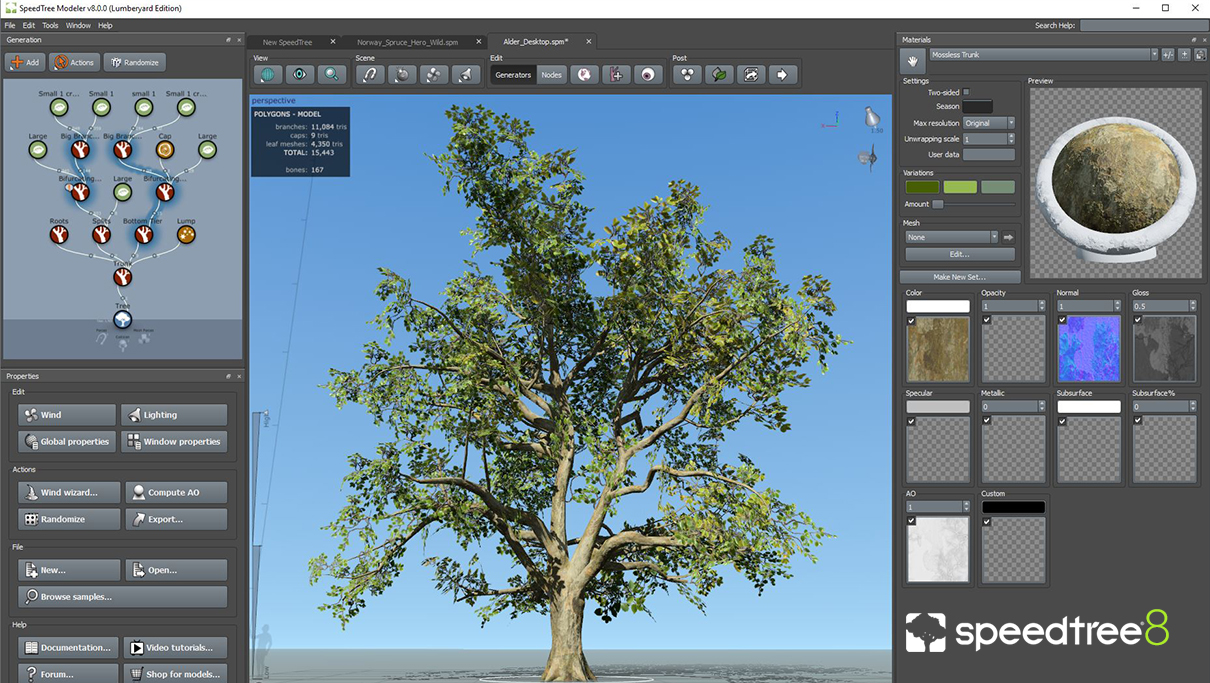
\includegraphics[scale=0.25]{speed_tree.jpg}
\end{figure}
\end{frame}

\begin{frame}{Reconstruction}
The landscape is scanned with LIDAR
Computer vision methods are used to create point cloud
A tree structure can be reconstructed from it
\begin{figure}[hbtp]
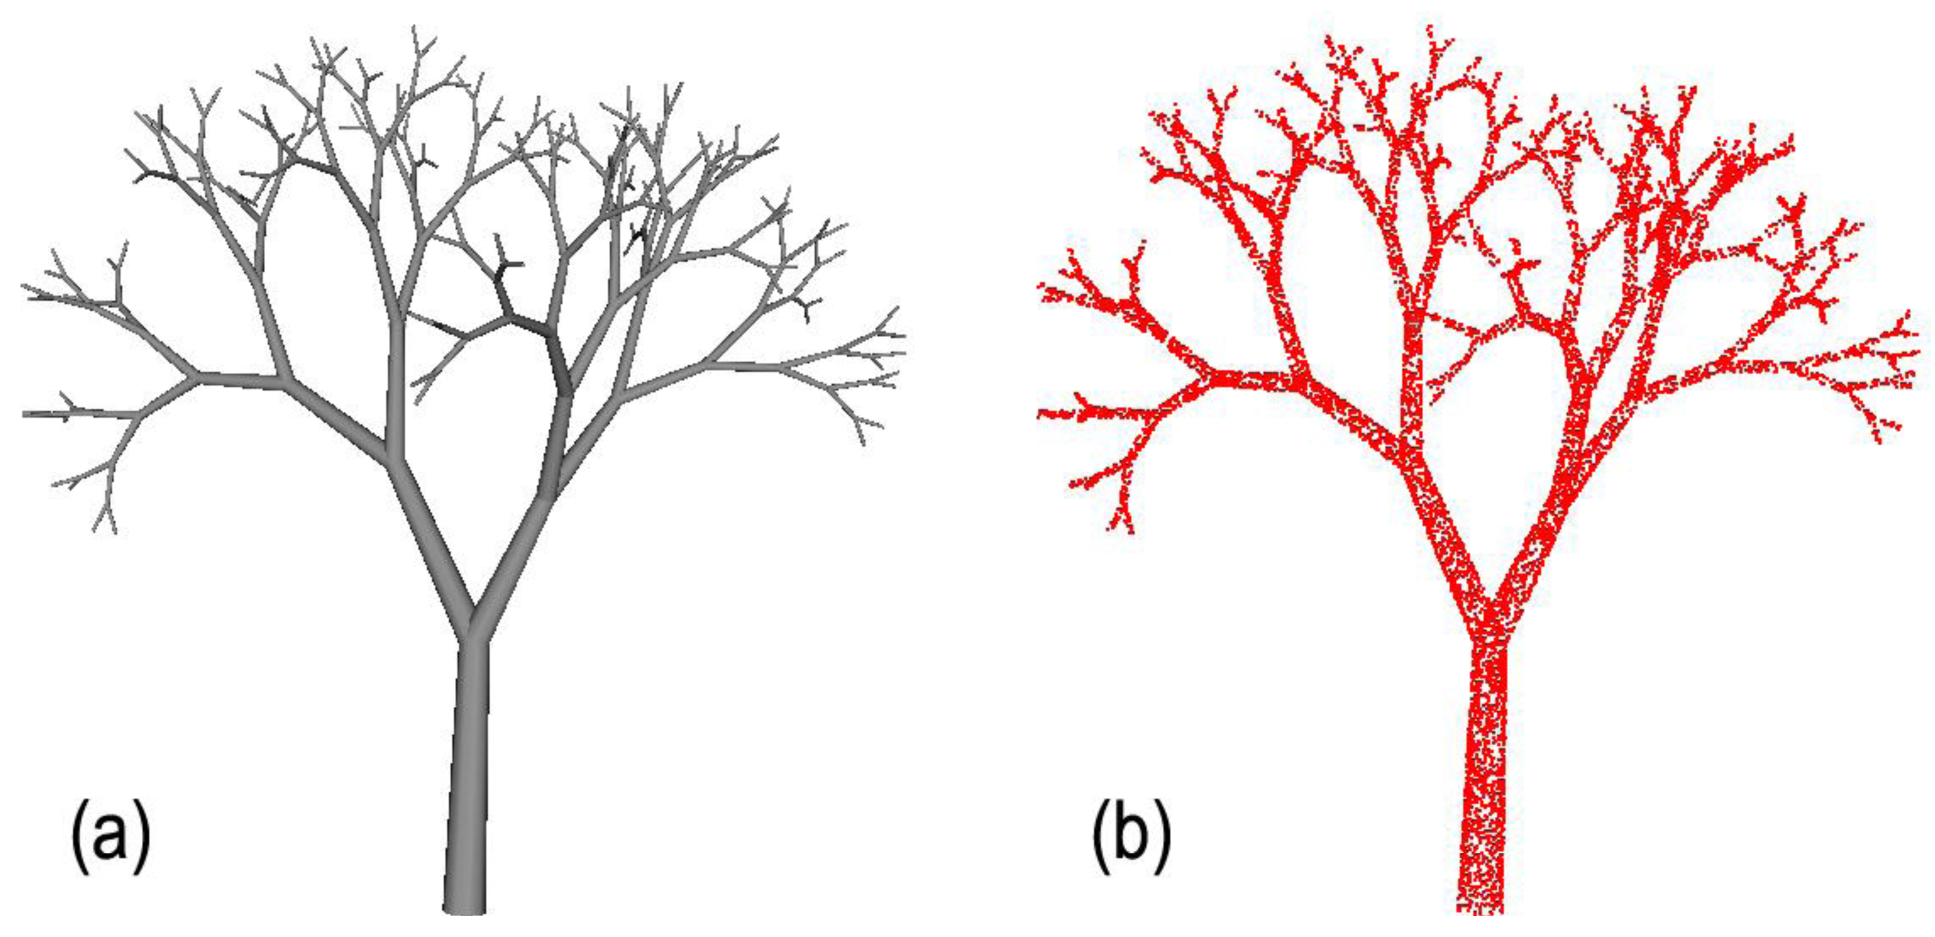
\includegraphics[scale=0.55]{recon.png}
\end{figure}
\end{frame}

\begin{frame}{The end}
Thank you for your attention!
\end{frame}
\end{document}